\documentclass[12pt]{article} 
\usepackage[utf8]{inputenc}
\usepackage[T2A]{fontenc}
\usepackage{amsthm}
\usepackage{amssymb}
\usepackage{blindtext}
\usepackage{amsmath}
\usepackage{tikz} 
\usepackage{listings}
\usepackage{xcolor}
\usepackage{float}
\usepackage{graphicx}
\graphicspath{ {./image} }

\title{Bioinformatics HW1}
\author{Ershov Ivan}
\date{October 2021}

\begin{document}

\maketitle

\paragraph{Задание 1. Геном Бактерии Micrococcus luteus}
\subparagraph{1. Какова длина генома (файл .fna)\\}
Для начала посчитаем количество строк в файле и вычтем из этого числа 1, то есть не будем учитывать первыую строку.\\\\
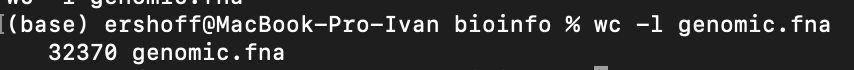
\includegraphics[width=\textwidth]{image/Image1.png}\\
Получаем $32370 - 1 = 32369$ строк.\\
Теперь посчитаем количество вхождений букв A, T, G, C и N.\\
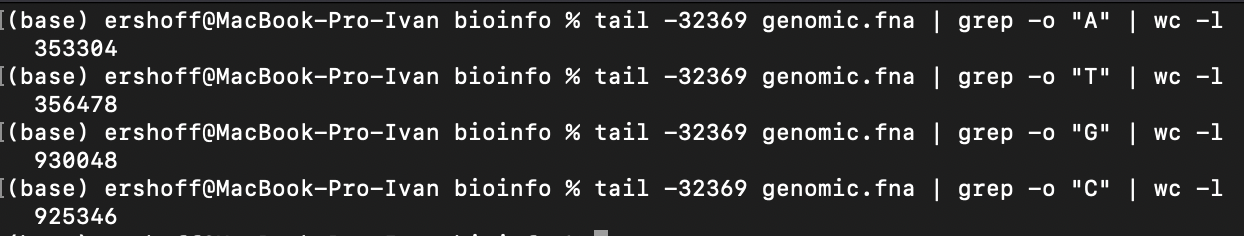
\includegraphics[width=\textwidth]{image/image2.png}\\
Полученные числа сложим и получим ответ:\\ $353304 + 356478 + 930048 + 925346 = 2'565'176$\\\\
Ответ: $2'565'176$

\subparagraph{2. Сколько генов, кодирующих белки?\\}
Просто посчитаем в терминале:\\
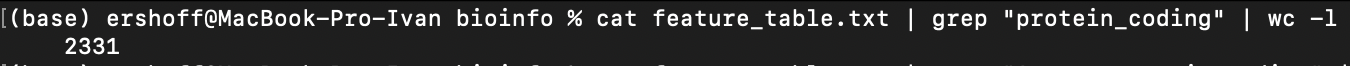
\includegraphics[width=\textwidth]{image/image3.png}\\
Ответ: $2331$
\pagebreak

\subparagraph{3. Сколько рнк-генов?\\}
Просто посчитаем в терминале:\\
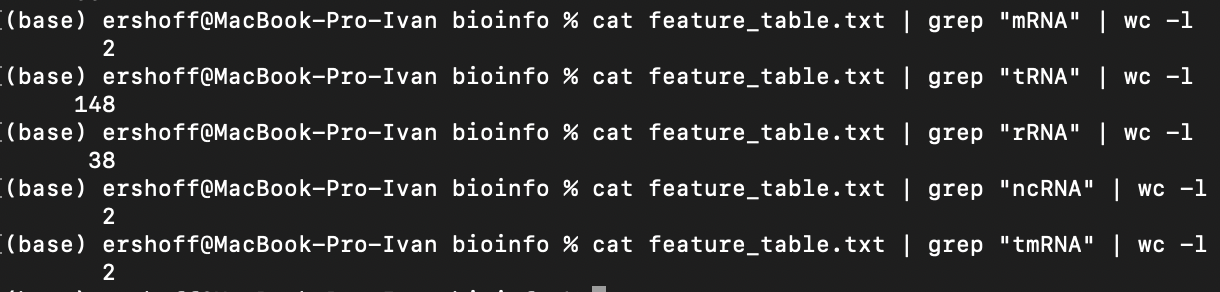
\includegraphics[width=\textwidth]{image/image4.png}\\
И просуммируем:\\
$2 + 148 + 38 + 2 + 2 = 192$\\
Ответ: $192$

\subparagraph{4. Сколько транскрипционных факторов?\\}
Просто посчитаем в терминале:\\
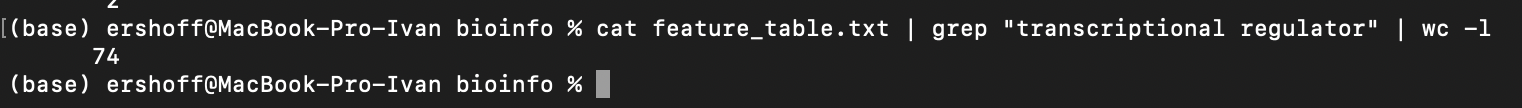
\includegraphics[width=\textwidth]{image/image5.png}\\
Ответ: 74

\subparagraph{5. Сколько транспортных белков (ABC transporters)?\\}
Просто посчитаем в терминале:\\

\includegraphics[width=\textwidth]{image/image6.png}\\
Ответ: 98

\subparagraph{6. Сколько tRNA?\\}
Просто посчитаем в терминале:\\
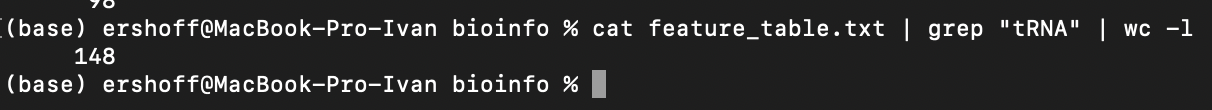
\includegraphics[width=\textwidth]{image/image7.png}\\
Ответ: 148

\pagebreak
\subparagraph{7. Сколько закодировано субъединиц АTP-synthase?\\}
Просто посчитаем в терминале:\\
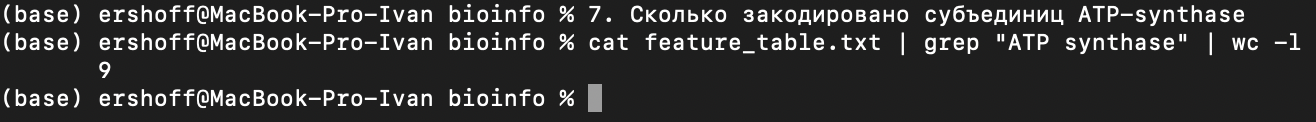
\includegraphics[width=\textwidth]{image/image8.png}\\
Ответ: 9

\subparagraph{8. Сколько генов закодировано на положительном, а сколько на отрицательном стренде?\\}
Посчитаем количество строк, начинающихся на "gene" и заканчивающихся на '+' и '-' и вычтем из полученных чисел количество псевдогенов для '+' и '-' генов соответсвенно:\\
Начнем с положительных стрендов:\\
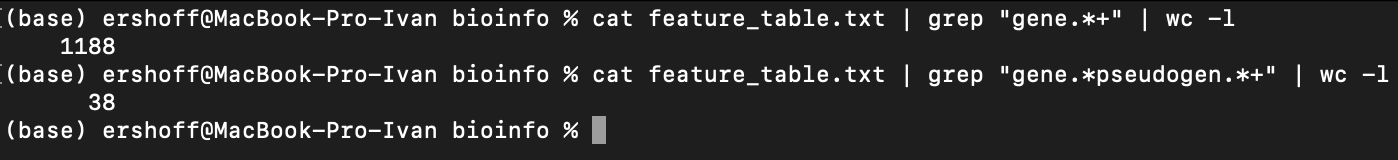
\includegraphics[width=\textwidth]{image/image9.png}\\
В итоге получаем $1188 - 38 = 1150$ генов на положительном стренде.\\\\
Теперь для отрицательных стрендов:\\
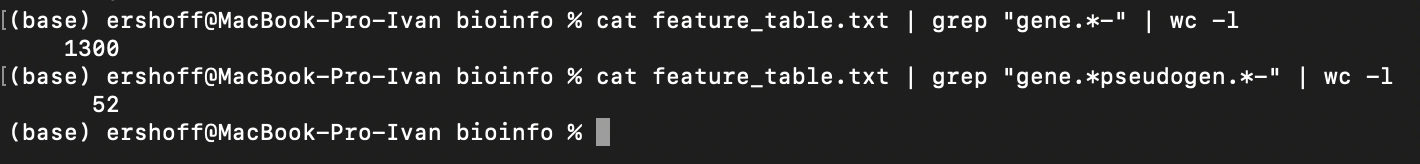
\includegraphics[width=\textwidth]{image/image10.png}\\
В итоге получаем $1300 - 52 = 1248$ генов на отрицательном стренде.\\\\
Ответ: 1150 и 1248 соответсвенно

\pagebreak
\paragraph{Задание 2. Ген Человека CDC42BPB}

\subparagraph{1. В геномном браузере UCSC отобразить все изоформы гена, а также SNPs (common and clinically relevant), участки консервативности среди позвоночных и транспозоны. Сохранить скриншот в виде графического файла.\\}
В UCSC установим следующие расширения:
\begin{itemize}
\setlength\itemsep{0.05em}
\item Gencode v36
\item Old UCSC Genes(full) (для изоформ)
\item Common SNPs(151) dense (для сommon SNP)
\item Flagged SNPs(151) dense (для clinically relevant SNP)
\item Conservation full (для учатков консервативности среди позвоночных)
\item Repeatmasker full (для транспозонов)
\item остальные расширения уберем (hide)
\end{itemize}
В итоге получаем:
\begin{figure}[H]
\centering
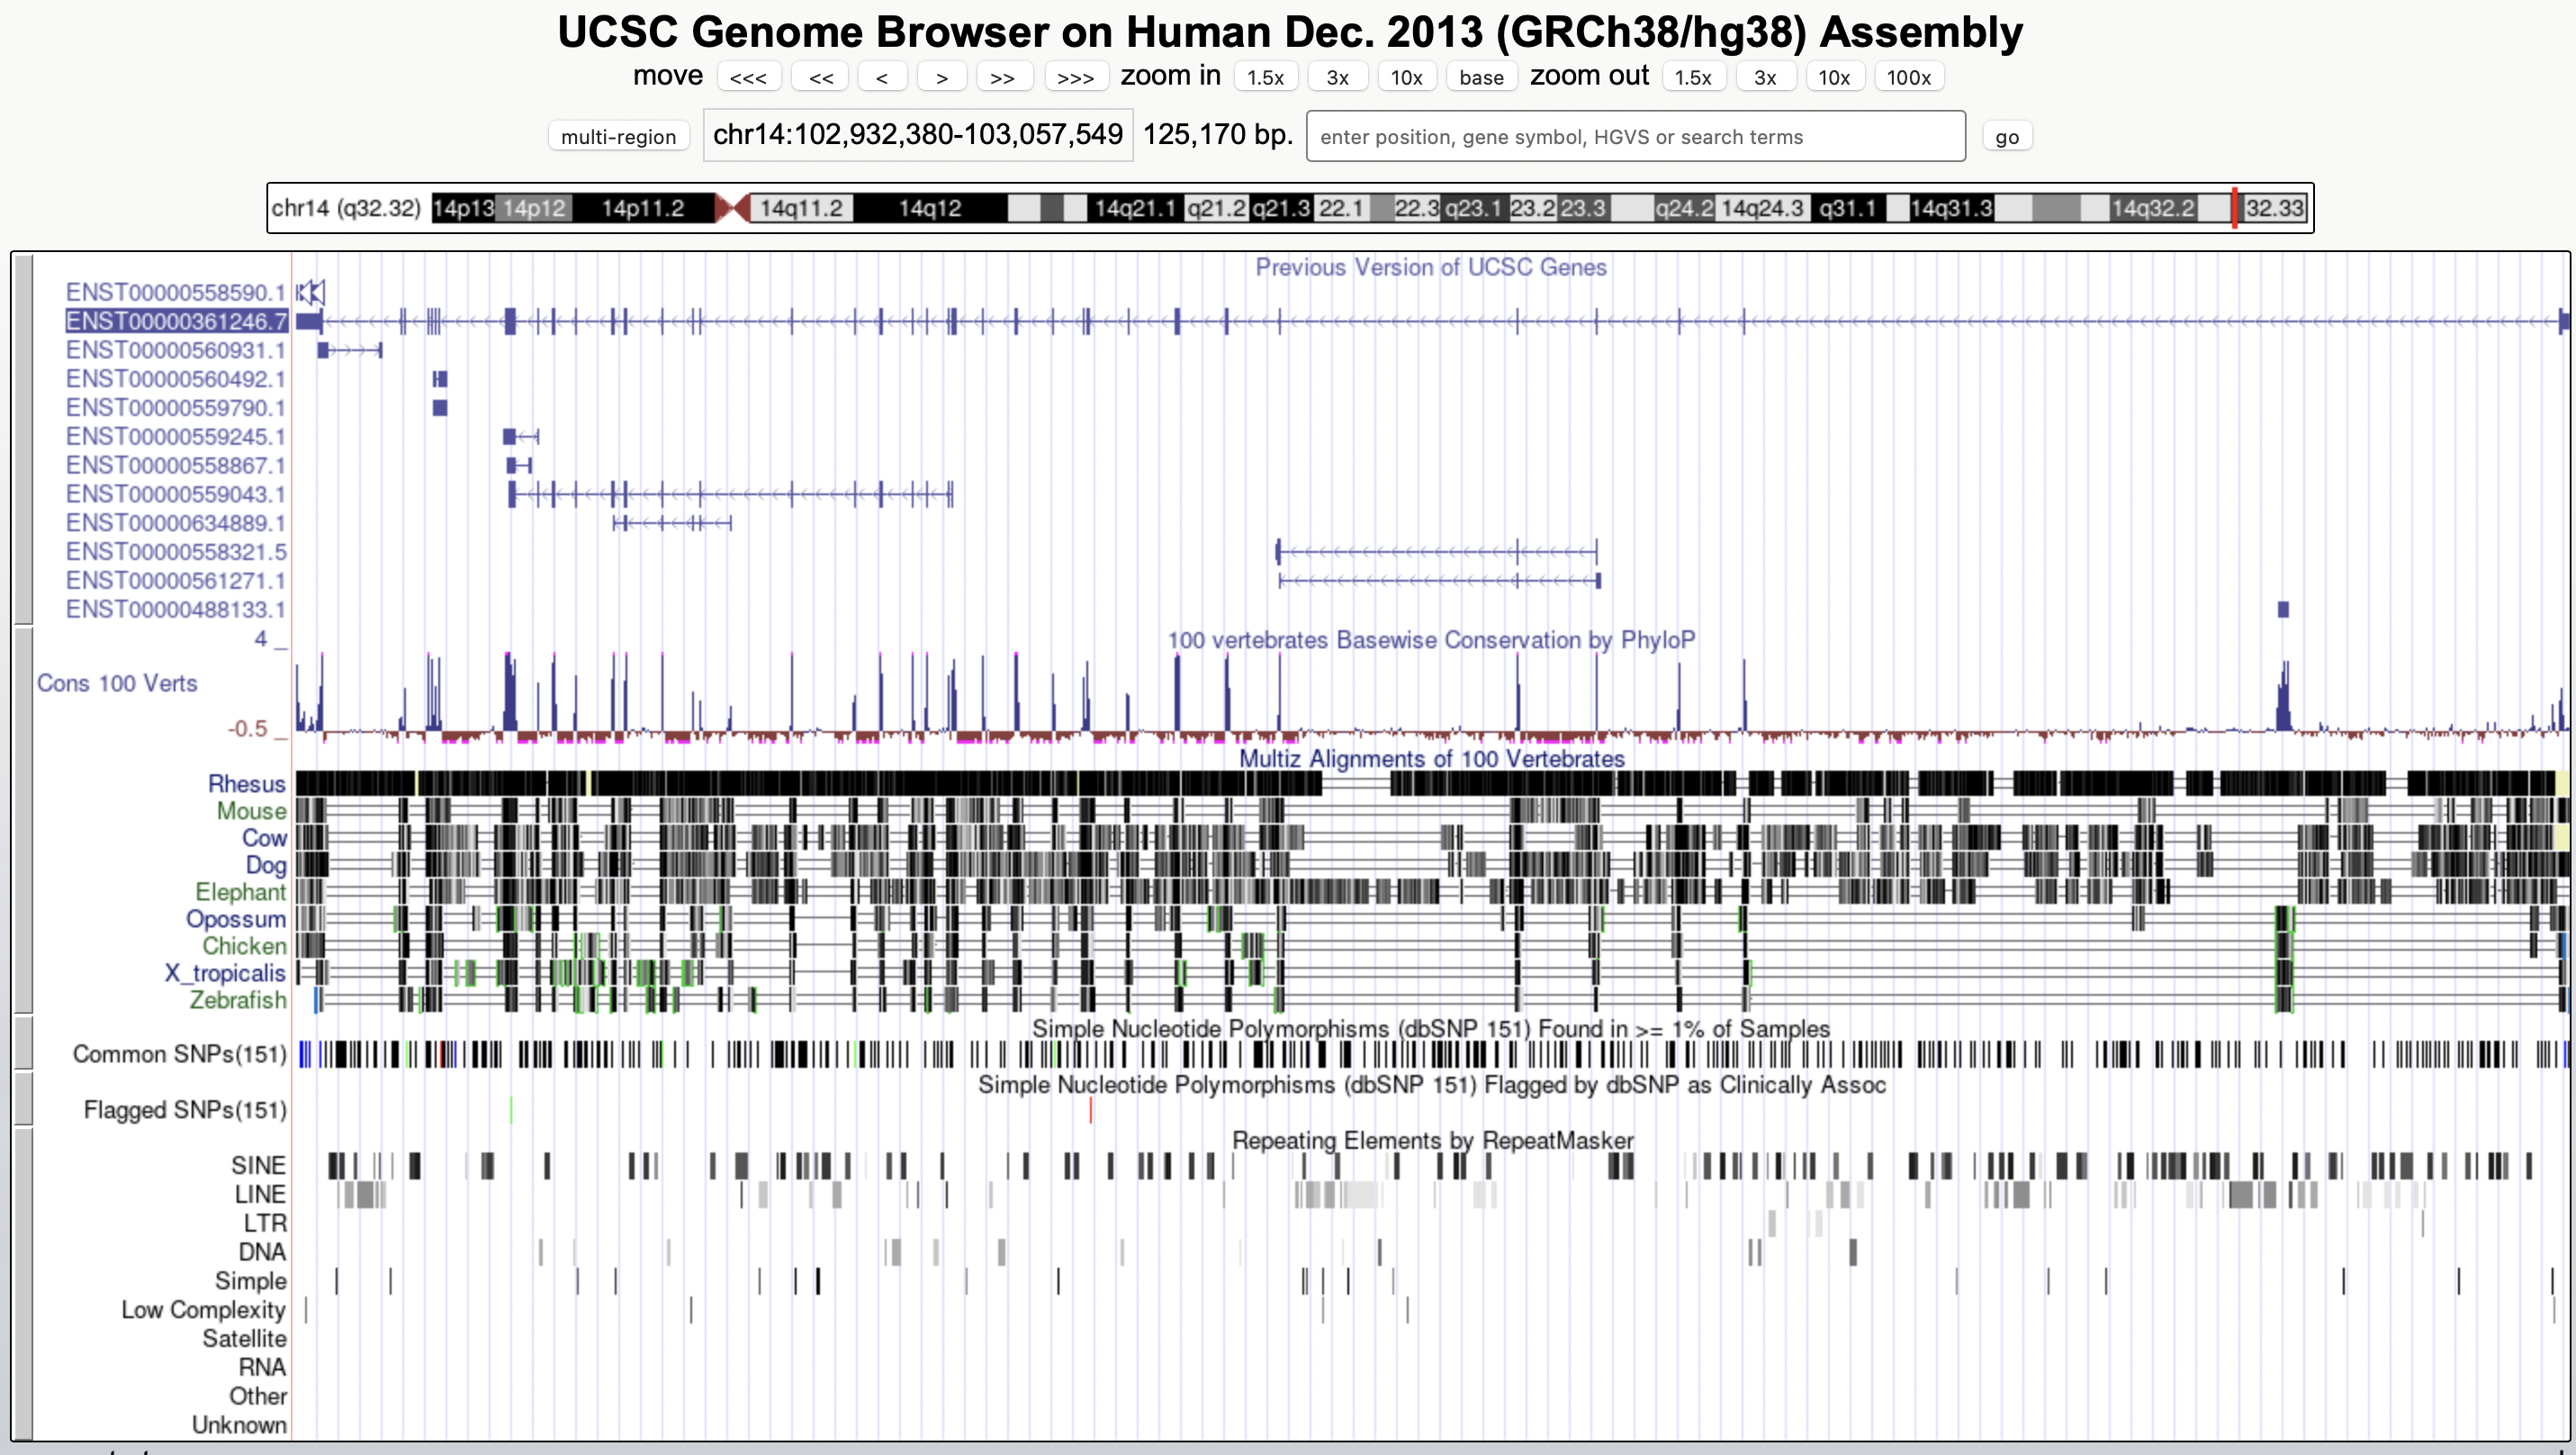
\includegraphics[width=17cm]{image/image11.png}
\end{figure}
\pagebreak

\subparagraph{2. Отобрать в табличном виде и сохранить в текстовый файл все изоформы генов, попавших в заданный участок\\}
Чтобы получить таблицу с изоформами, в Genome Browser выберем только Gencode v36 и Old UCSC Genes(full), а все остальное hide. Теперь зайдем во вкладку Tools $\rightarrow$ Table Browser и выберем следующее:
\begin{figure}[H]
\centering
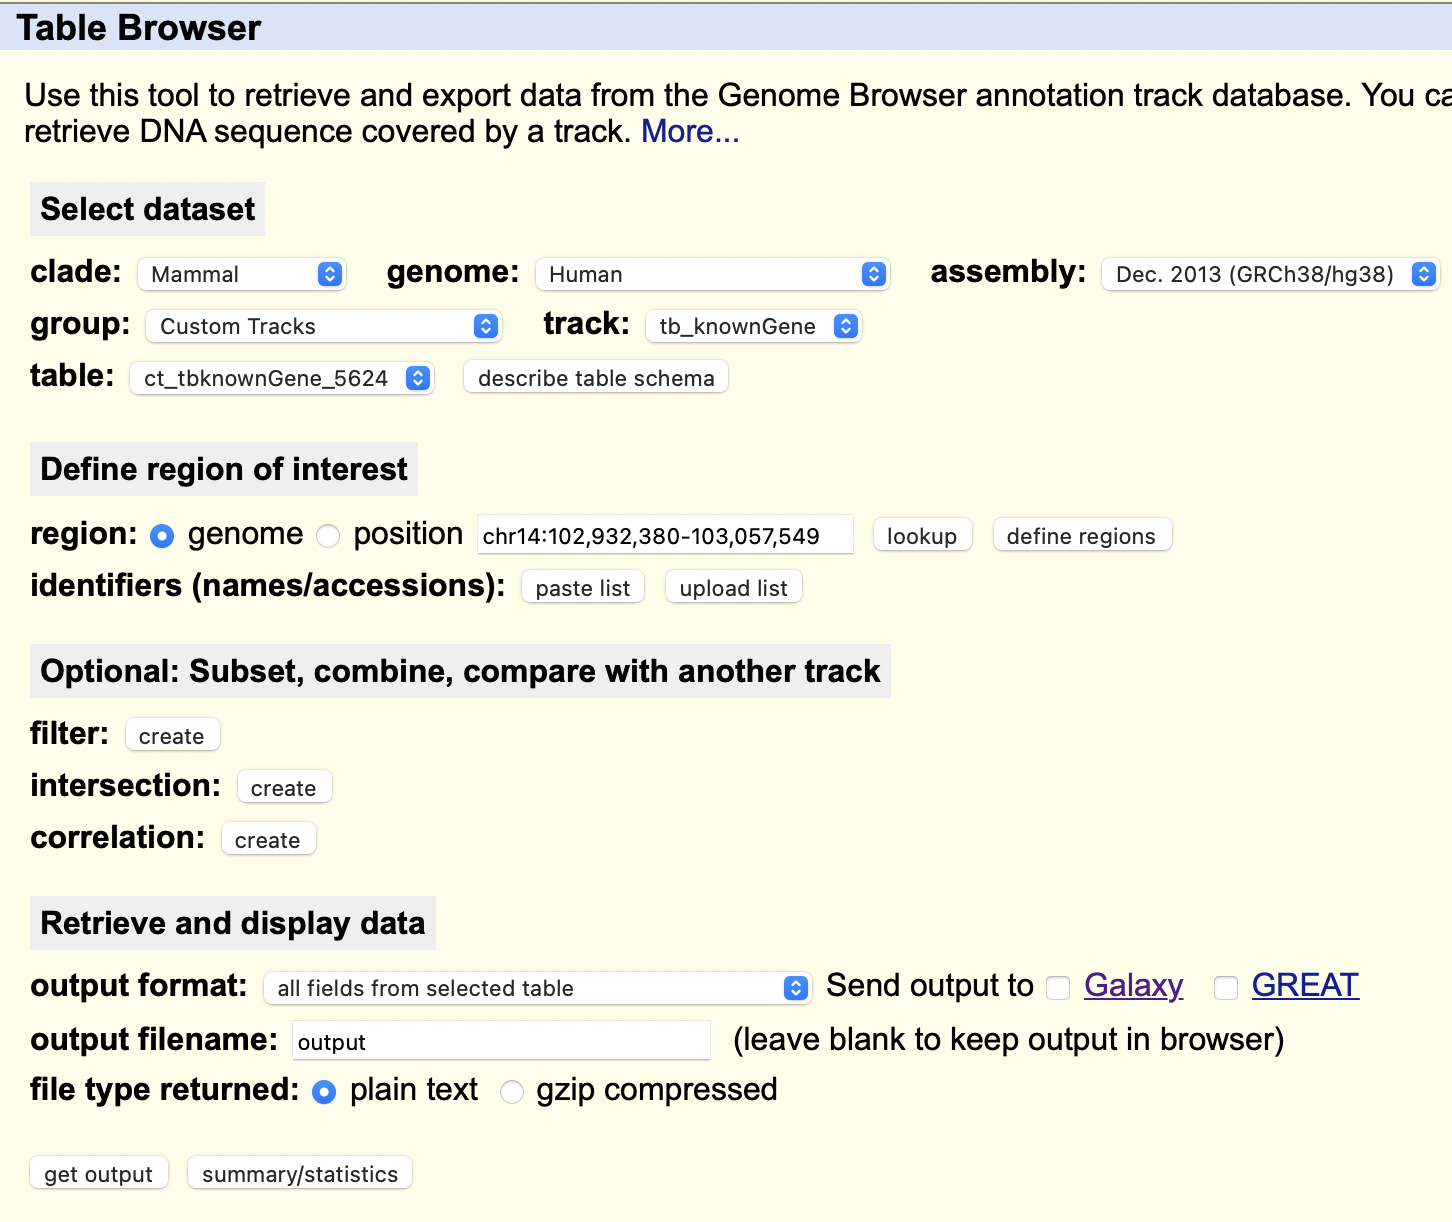
\includegraphics[width=15cm]{image/image13.png}
\end{figure}
Чтобы сохранить таблицу в виде тексового файла, укажем output filename и plain text\\\\\\\\\\
В итоге получаем таблицу: \\\\
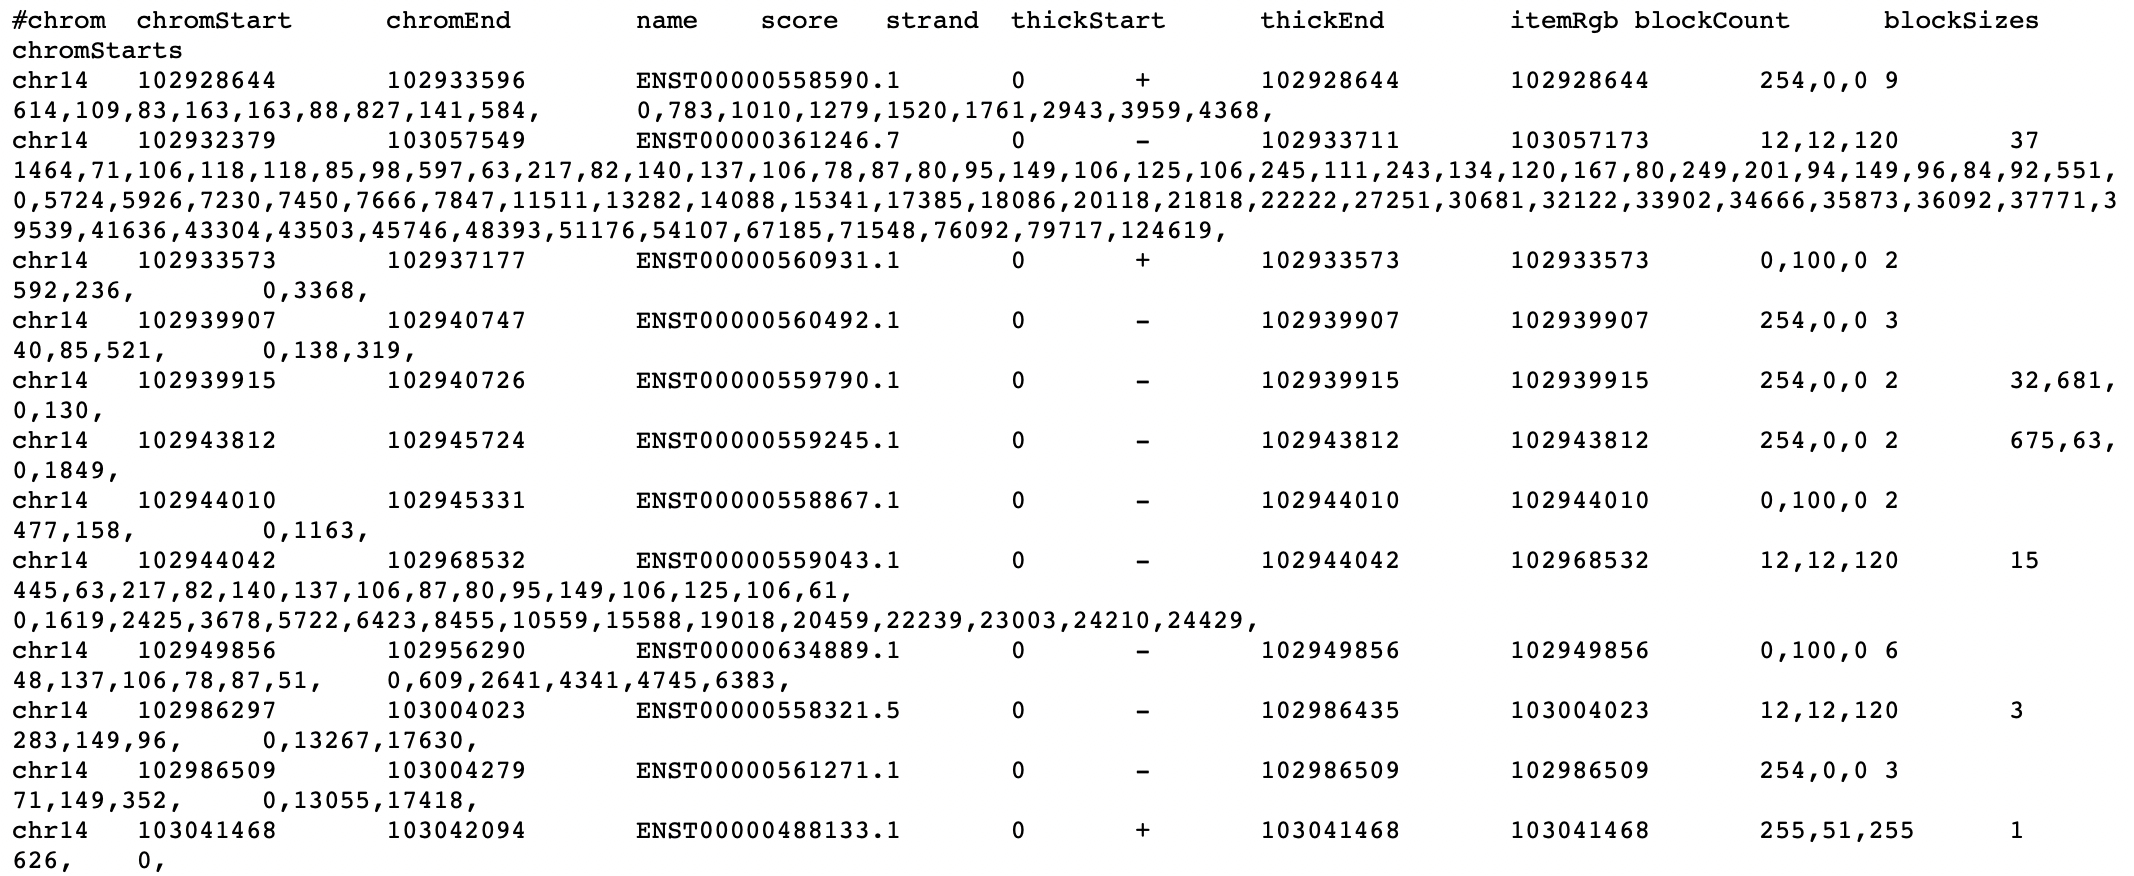
\includegraphics[width=17cm]{image/image12.png}

\subparagraph{3. Отобрать координаты только экзонов и только интронов для заданного участка.\\}
Tools $\rightarrow$ Table Browser $\rightarrow$ выберем BED в output format $\rightarrow$ get output $\rightarrow$ Exon plus / Intron plus $\rightarrow$ get BED\\
Получаем таблицы, где во втором столбце координата начала, а в третьем столбце координата конца экзона/интрона.\\\\
(Скриншоты полностью не поместились)\\

\newpage
Экзоны:\\
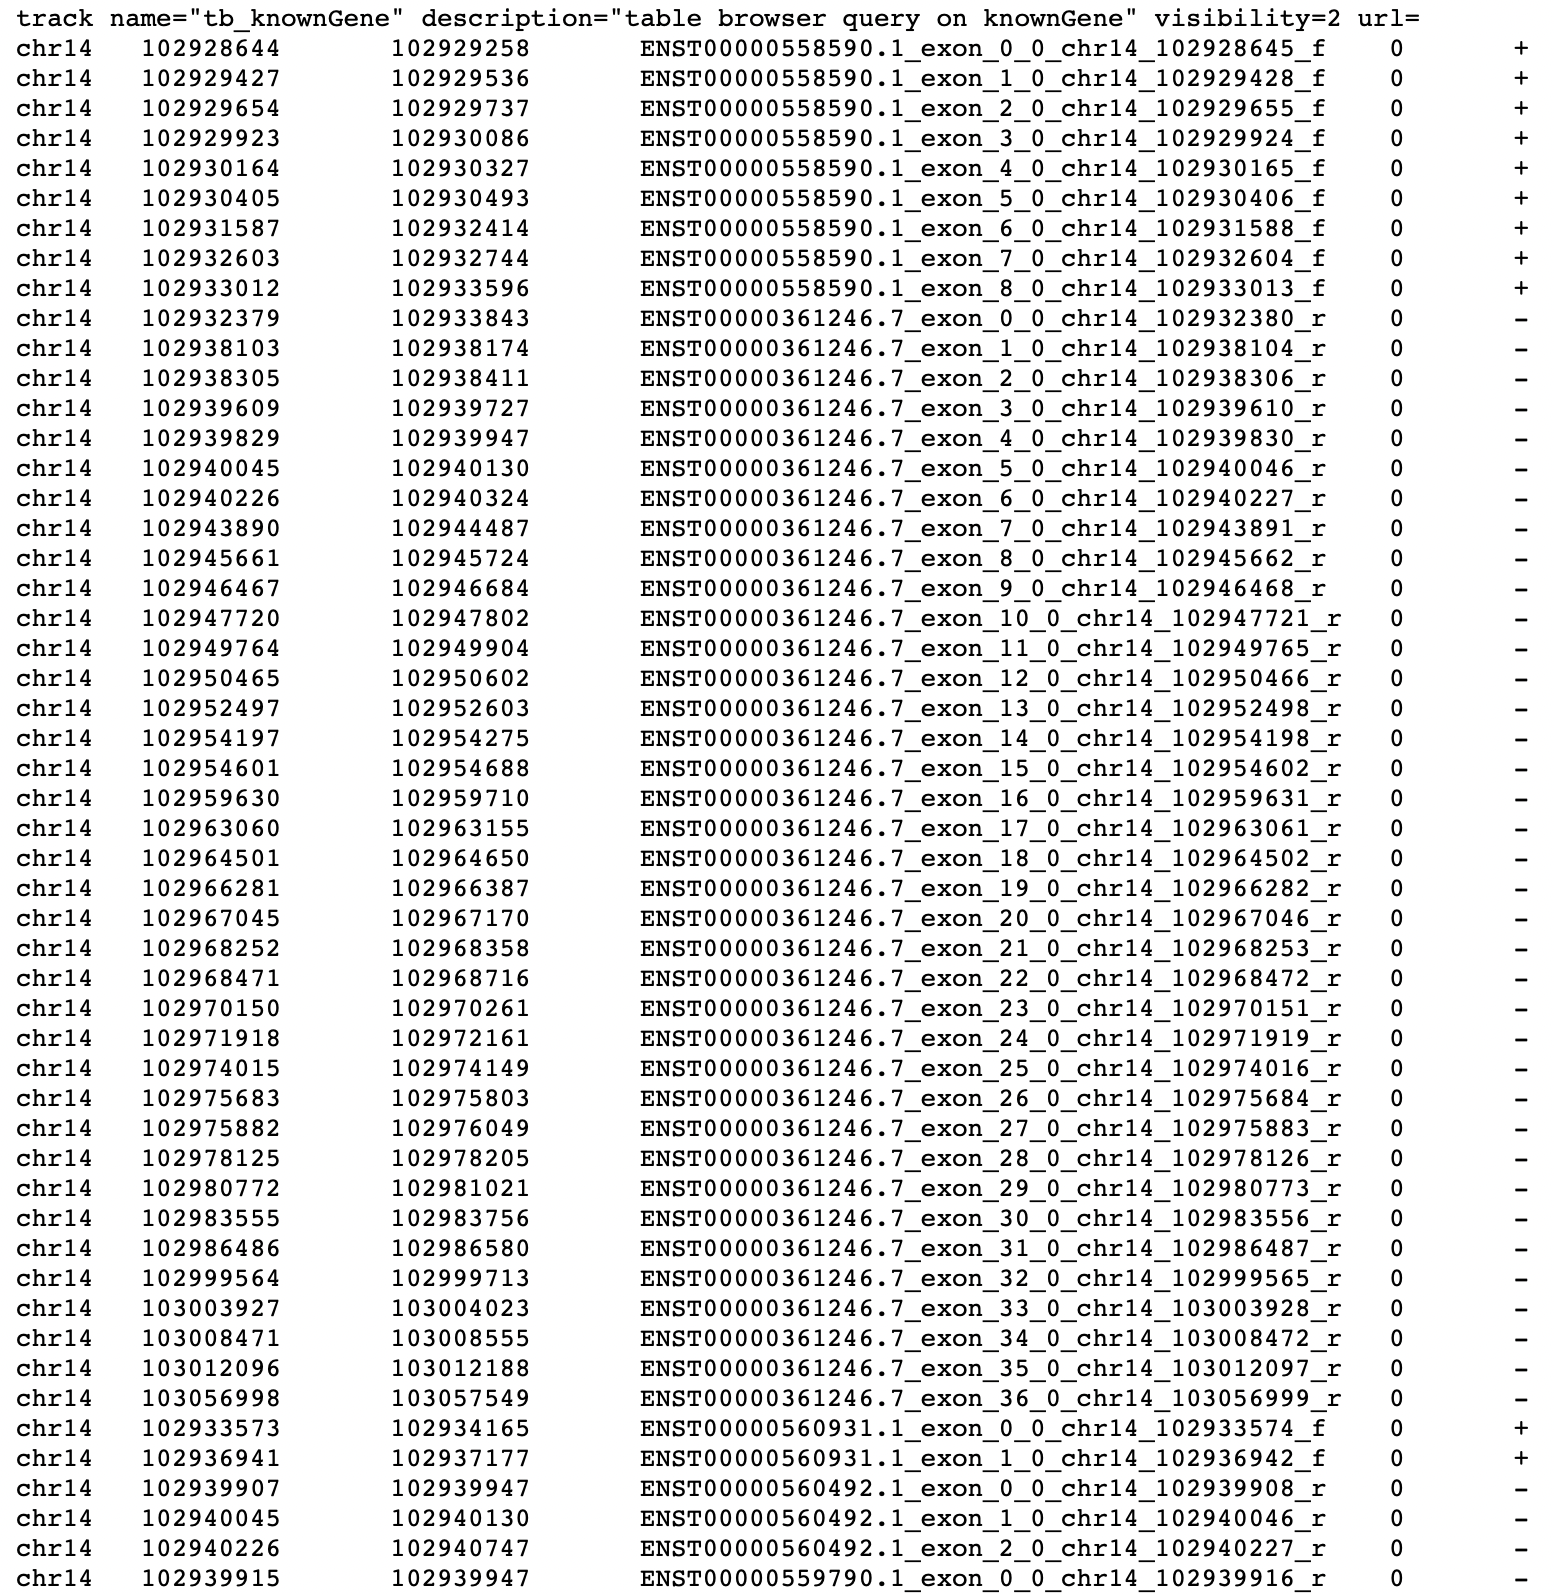
\includegraphics[width=15cm]{image/image14.png}\\
\newpage
Интроны:\\
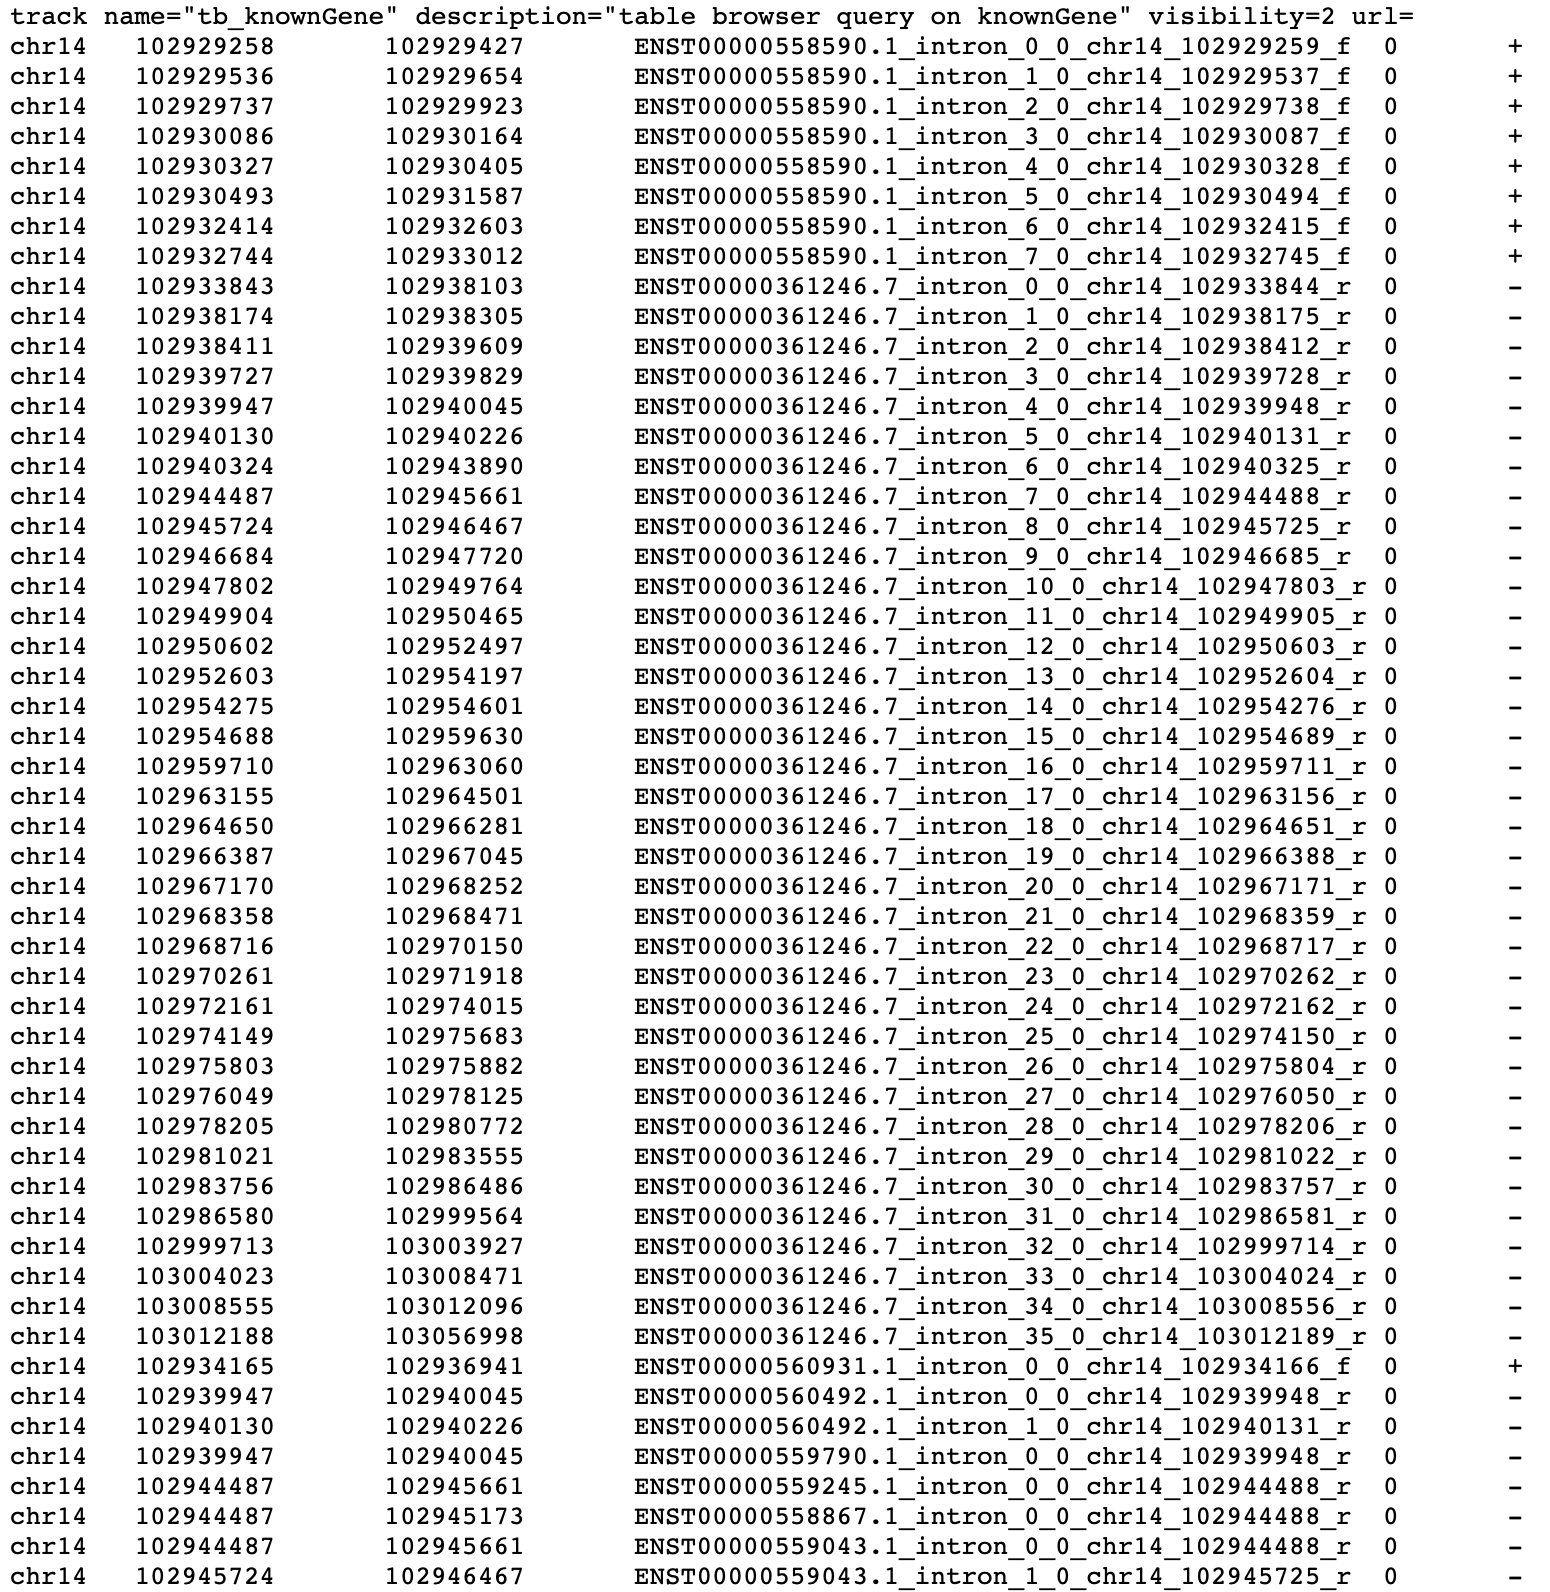
\includegraphics[width=15cm]{image/image15.png}
\newpage

\subparagraph{4. Ответить письменно, в какие участки гена попадают clinically relevant SNPs.\\}
Для удобства выведем только сlinically relevant SNPs.\\
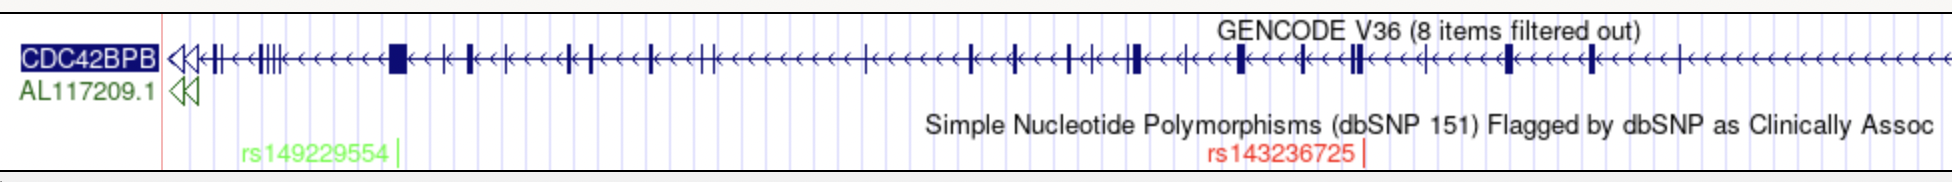
\includegraphics[width=15cm]{image/image16.png}\\
(зеленым и красным отмечены сlinically relevant SNPs)\\\\
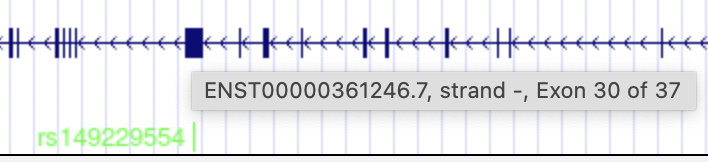
\includegraphics[width=7cm]{image/image17.png}
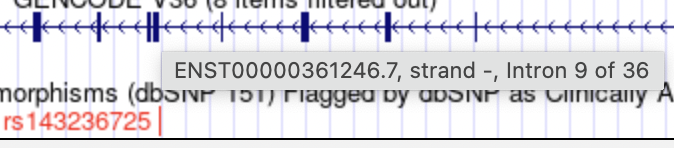
\includegraphics[width=7cm]{image/image18.png}\\\\
Мы видим, что всего 2 clinically relevant SNPs попадают на ген: один попадает на интрон, другой на экзон.

\subparagraph{5. Ответить письменно, в какие участки гена попадают транспозоны.\\}
Чтобы отобразить транспозоны, выберем только Gencode v36 pack и RepeatMasker full.\\
Транспозоны попадают как и на экзоны, так и на интроны:\\
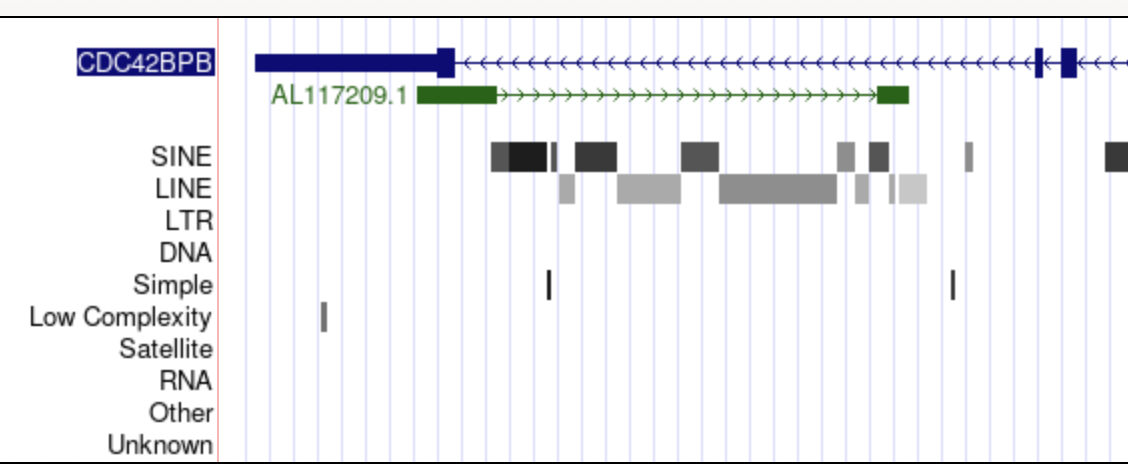
\includegraphics[width=15cm]{image/image19.png}\\
(Из скриншота это явно видно)
\end{document}